% !TeX root = ../main.tex
% !TeX encoding = UTF-8
% !TeX spellcheck = en_US
% !TeX program = pdflatex

\section{Evaluating Flat Segmentations}
\subsection{Pairwise Clustering}
For evaluating how the segments are labeled, metrics are inspired by casting the segmentation problem as a clustering problem, where different atomic structural units (audio frame, beat, or measure) are clustered according to their segment labels.
Pairwise Frame Clustering (PFC) score is such an adaptation: it uses the same concept of precision and recall as above, but focusing on whether pairs of frames are labeled consistently~\cite{levy2008structural}.

Using $L: t \rightarrow \{y_1, \ldots, y_k\}$ to denote the reference label at time $t$, the set of time point pairs $\rho = \{(u, v)|L(u)=L(v)\}$ is defined as all $u, v$ pairs that are labeled identically by $L$.

Pairwise frame clustering metrics are then defined as follows: 
\begin{align*}
\text{PFC}_R = \frac{|\rho_\text{ref} \cap \rho_\text{est}|}{|\rho_\text{ref}|}&, \quad
\text{PFC}_P = \frac{|\rho_\text{ref} \cap \rho_\text{est}|}{|\rho_\text{est}|} \\
\text{PFC}_F = &\frac{2}{\frac1{\text{PFC}_R} + \frac1{\text{PFC}_P}}
\end{align*}
We can visualize the labels of a segmentation by plotting its Annotation Agreement Map (AAM) $A(u, v) = [(u, v) \in \rho]_\mathbbm{1}$ as is done in figure~\ref{fig:flat_anno_meet}.
Notice $|\rho|$ represents the number of non zero entries in $A(u, v)$, and $|\rho_\text{ref} \cap \rho_\text{est}|$ represent the number of pairs in the overlapping areas between $A_\text{ref}(u, v)$ and $A_\text{est}(u, v)$.

% \begin{figure}
%     \centering
%     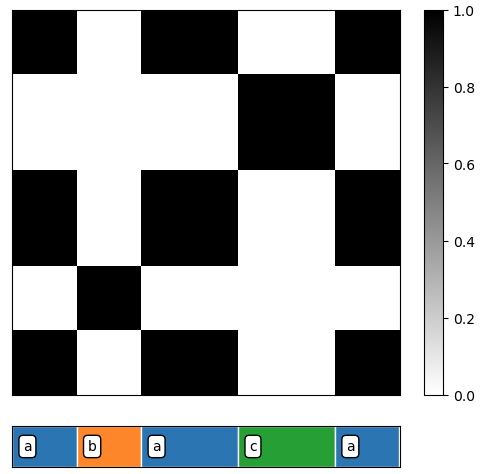
\includegraphics[width=0.5\linewidth]{content/figs/flat_anno_meet.png}
%     \caption{Annotation Agreement Map for the simple Rondo structure represented at the bottom}
%     \label{fig:flat_anno_meet}
% \end{figure}

\subsection{V-measure}
Inherent from its definition, the PFC metric favors coarser segmentations where its $A_\text{est}(u, v) = 1$ for large ranges of $u$ and $v$.
This incentivized the adoption of V-measure, another clustering metric, which is the current standard for comparing flat segmentations' labels~\cite{lukashevich2008towards}.
Instead of simply counting occurrences, V-measure looks at the normalized entropy of the true labels conditioned on their estimated label, and vice versa.
For a labeled segmentation $L(t)$ using a set of $k$ labels $\gamma = \{y_1, \ldots, y_k\}$, the entropy of the label distribution can be examined by sampling randomly along its duration:
$$\mathbb{H}(L(t)) = \underset{{y\in\gamma}}{\mathbb{E}}[-\log\mathbb{P}(L(t) = y)]$$
$\mathbb{H}(L(t))$ measures the uncertainty in the distribution defined by $\mathbb{P}(L(t))$ and equals to 0 when the distribution is deterministic (i.e. $L(t) = y_1$ for all $t$). 

$$\mathbb{H}(L_\text{ref} | L_\text{est}) = \underset{y\in\gamma}{\mathbb{E}}[\mathbb{H}(L_\text{ref} | L_\text{est}(t) = y)]$$
is the conditional entropy, which looks at the entropy of reference frame labels only when they receive the same label in the estimate segmentation.
Conceptually, the conditional entropy estimates the amount of uncertainty left in predicting the reference labels given the estimate segmentation.
When the uncertainty for reference label is low given the estimated label, the estimate recalls the labeling information presented in the reference.

V-measure normalizes the conditional entropy by the marginal entropy of the segment labels to calibrate scores for segmentations that have different number of distinct labels.
\begin{align*}
\text{V}_R = 1 - \frac{\mathbb{H}(L_\text{ref} | L_\text{est})}{\mathbb{H}(L_\text{ref})}&, \quad
\text{V}_P = 1 - \frac{\mathbb{H}(L_\text{est} | L_\text{ref})}{\mathbb{H}(L_\text{est})} \\
\text{V}_F = &\frac{2}{\frac1{\text{V}_R} + \frac1{\text{V}_P}}
\end{align*}
